\documentclass{beamer}
\usetheme{Madrid}
\usecolortheme{beaver}

\usepackage{subcaption}

\title{Teacher Grading and Value-Added: \\ Evidence From Chicago}
\author{Roy McKenzie}
\institute{University of Chicago - Department of Economics}
\date{May 12, 2021}

\begin{document}

\frame{\titlepage}

\begin{frame}
\frametitle{What We Know}
\begin{itemize}
	\item Grades are a \textbf{strong} predictor of student outcomes 
	\item Grades is non-standardized, and there is lots of variation
	\item This is observable is student experience 
\end{itemize}
\end{frame}
%% Set the stage - TALK ABOUT CONSORTIUM RESEARCH

\begin{frame}
\frametitle{What We Want to Know}
What effect do a teacher’s grading practices have on their students’ long-term outcomes? That is, what is the causal effect of having a \textbf{``easy-A''}teacher vs. a \textbf{``hard grader''}? \\~\\ \pause

Why this is important: \pause
\begin{itemize}
	\item Grade reliability \pause
	\item Equity 
\end{itemize}

Why this is hard: \pause
\begin{itemize}
	\item Non-random teacher assignment \pause
	\item Disentangling Grades
\end{itemize}
\end{frame}
%% Talk about policy relevance

\begin{frame}
\frametitle{What I Can Try and Answer}
How is the \textbf{non-persistent component} of teacher's grading correlated with their students' long-term outcomes? \\~\\ \pause

To do this:
\begin{itemize}
	\item First-differenced outcomes \pause
	\item Novel assumptions
\end{itemize}
\end{frame}
%% Talk about what we can't do!!! We're going to call this a grade effect, but be careful. 

\begin{frame}
\frametitle{Setting and Data - Chicago Public Schools}
% Things good for policy and good for me

Chicago Public Schools:
\begin{itemize}
	\item 20,000 teachers, 350,000 students - Lots of variation!
	\item Relative stability 
	\item Common transition elementary to high school 
\end{itemize}


Scope:
\begin{itemize}
	\item Freshman year - pivotal for CPS, good for random assignment 
	\item Core classes - linked to later outcomes, consistent across students 
\end{itemize}

Data:
\begin{itemize}
	\item Longitudinal administrative data 
	\item Class-level data
	\item Long-term outcome data
	\item Main analytic sample is freshman classes from 2011-12 to 2013-14
\end{itemize}
\end{frame}

%% Talk about main idea here
\begin{frame}
\frametitle{Primary Model}

The primary model is given by
\begin{equation}
	\label{eqn:final}
	g_{it}-g_{i,t+1}=\nu_{j(it)} + \beta X_{it} + e_{it} + u_{i,t+1} 
\end{equation}
where 
\begin{itemize}
	\item $g_{it}$ is student $i$'s level of human capital in time $t$
	\item $j(it)$ is the teacher assigned to student $i$ in time $t$
	\item $\nu_{j(it)}$ is teacher $j(it)$'s idiosyncratic ``grade-effect'' 
	\item $X_{it}$ is a vector of student school and class level controls
	\item $e_{it}$ are unobserbved characteristics of a student's teacher in period $t$, net of the controls
	\item $u_{i,t+1}$ are unobserved characteristics of a student's teacher in period $t+1$, net of the controls
\end{itemize} 

\end{frame}

\begin{frame}
\frametitle{Three Necessary Assumptions for Identification}
\begin{alertblock}{Assumption 1 (Additivity)}
Assume the law of motion for human capital has a form given by 
			\[
				h_{it} = h_{i,t-1} + \gamma_{j(it)} 
			\]
where 
\begin{itemize}
	\item $h_{it}$ represents a student's human capital at the end of time $t$
	\item $\gamma_{j(it)}$ is teacher $j(it)$'s ``value-added'' effect on student learning
\end{itemize}  
\end{alertblock}
\end{frame}

\begin{frame}
\frametitle{Three Necessary Assumptions for Identification}
\begin{alertblock}{Assumption 2 (Random Assignment of Teacher $j(it)$)}
Assume that 
		\[
			\mathbb{E}[e_{it} \mid j(it)] = \mathbb{E}[e_{it}] = 0 
		\]
That is, students are not sorted to their period $t$ teacher based on unobservable determinants of a student's grade.
\end{alertblock}
\end{frame}

\begin{frame}
\frametitle{Three Necessary Assumptions for Identification}
\begin{alertblock}{Assumption 3 (Random Assignment of Teacher $j(i,t+1)$)}
 Assume that 
		\[
			\mathbb{E}[u_{i,t+1} \mid j(it)] = \mathbb{E}[u_{it}] = 0
		\]
	This assumption implies that the characteristics of a student's teacher in period $t+1$ which are not predicted by student observables are not related to determined by their teacher assignment in period $t$.
\end{alertblock}
\end{frame}

\begin{frame}
\frametitle{Estimation Results}

Estimated using a combination of fixed effects and empirical Bayes methods, split by subject/year:

\begin{figure}[H]
	\centering
	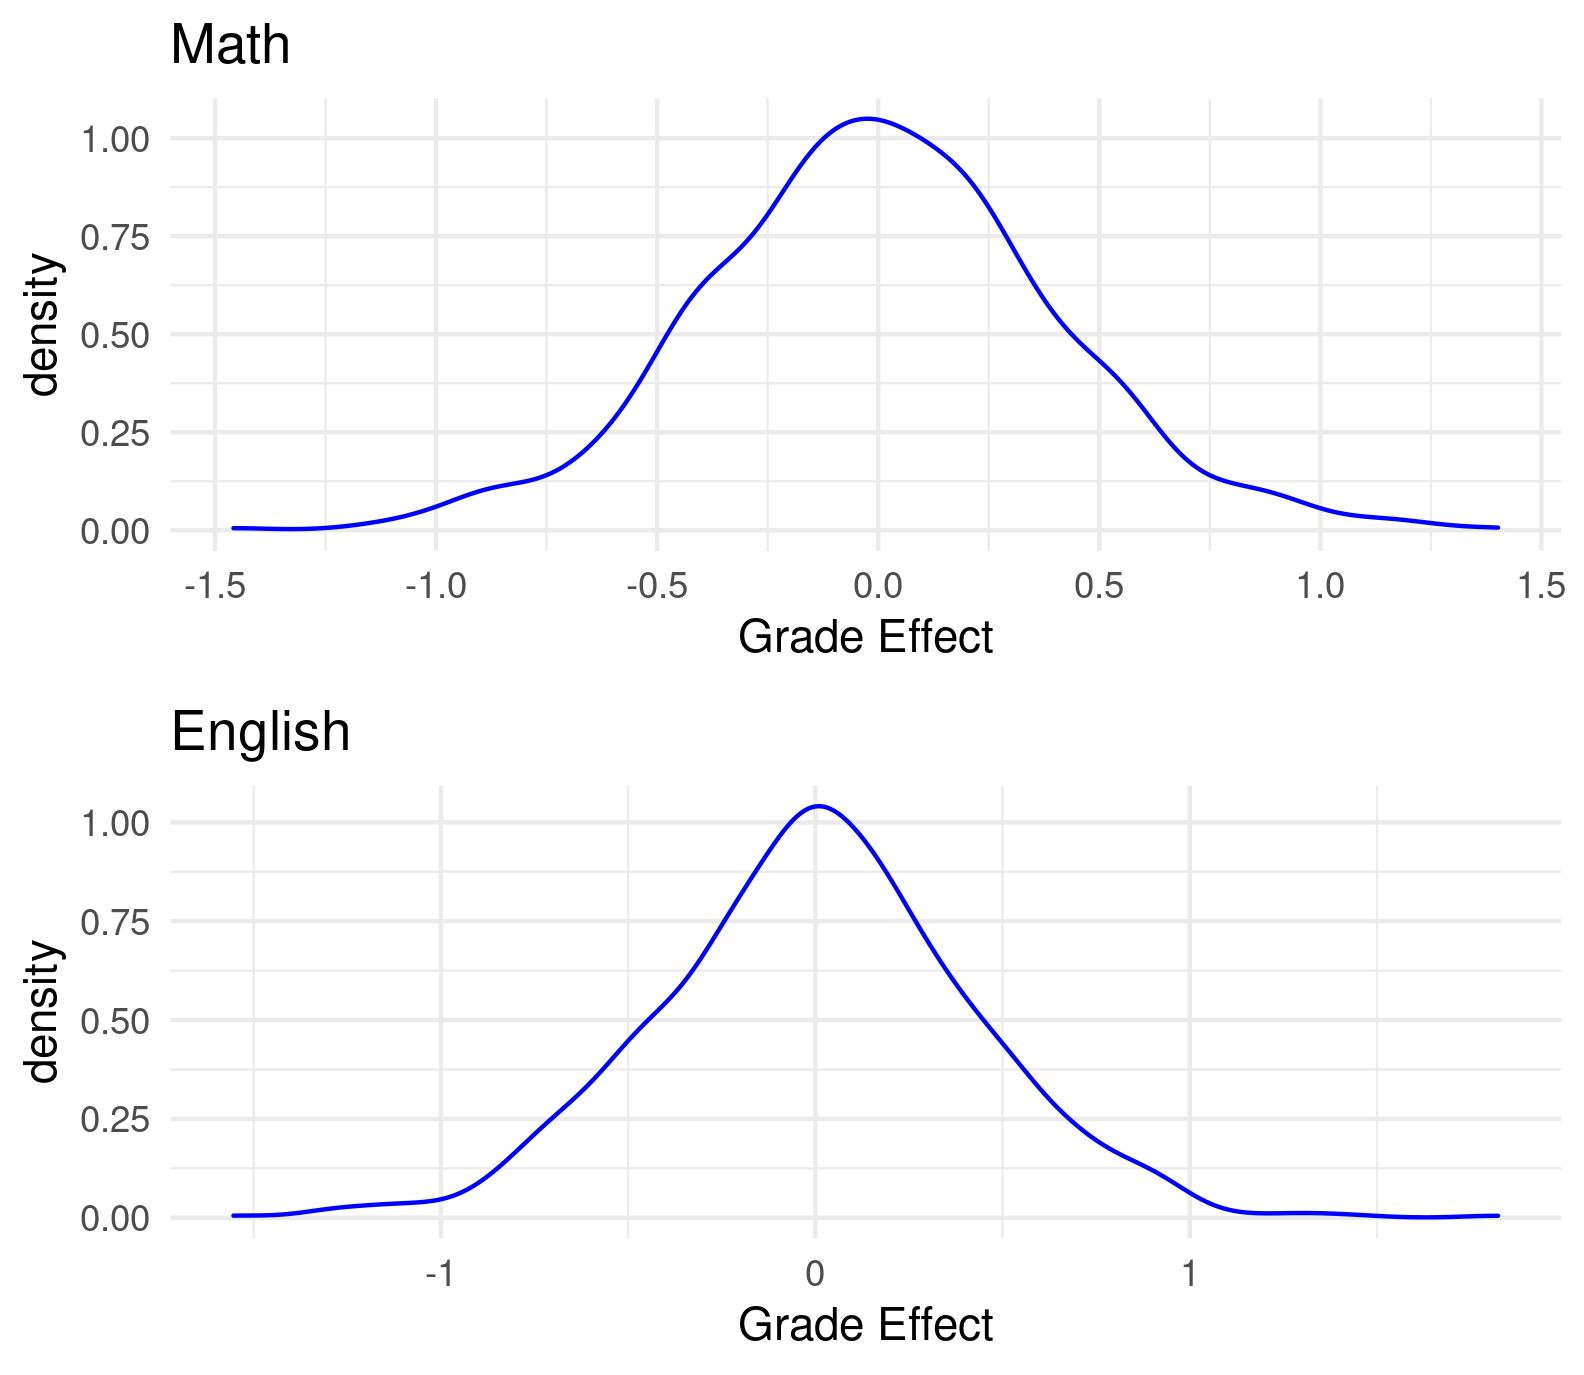
\includegraphics[width=.5\textwidth]{/Users/roymckenzie/Dropbox/Thesis/ECON/Output/Grade_Effect_Density.jpeg}
	\caption{Distribution of Estimated Grade Effects by Subject}
	\label{fig:ge_dist}
\end{figure}


\end{frame}

\begin{frame}
\frametitle{Links to Other Outcomes}

To find the relationship between these teacher grade-effects, we pool by year and use OLS to estimate 

\begin{equation}
	Y_{it}^* = \kappa \hat{\nu}_{j(it)}^{std} + Year_{t} + \psi_{it}
\end{equation}

where 

\begin{itemize}
	\item $Y_{it}^*$ represents the residualized outcome for student $i$
	\item $\hat{\nu}_{j(it)}^{std}$ is the estimated-grade effect
	\item $Year_{t}$ is a year fixed effect
\end{itemize}
\end{frame}


\begin{frame}
\frametitle{Links to Freshman Outcomes}

\begin{figure}
     \centering
     \begin{subfigure}[b]{0.3\textwidth}
         \centering
         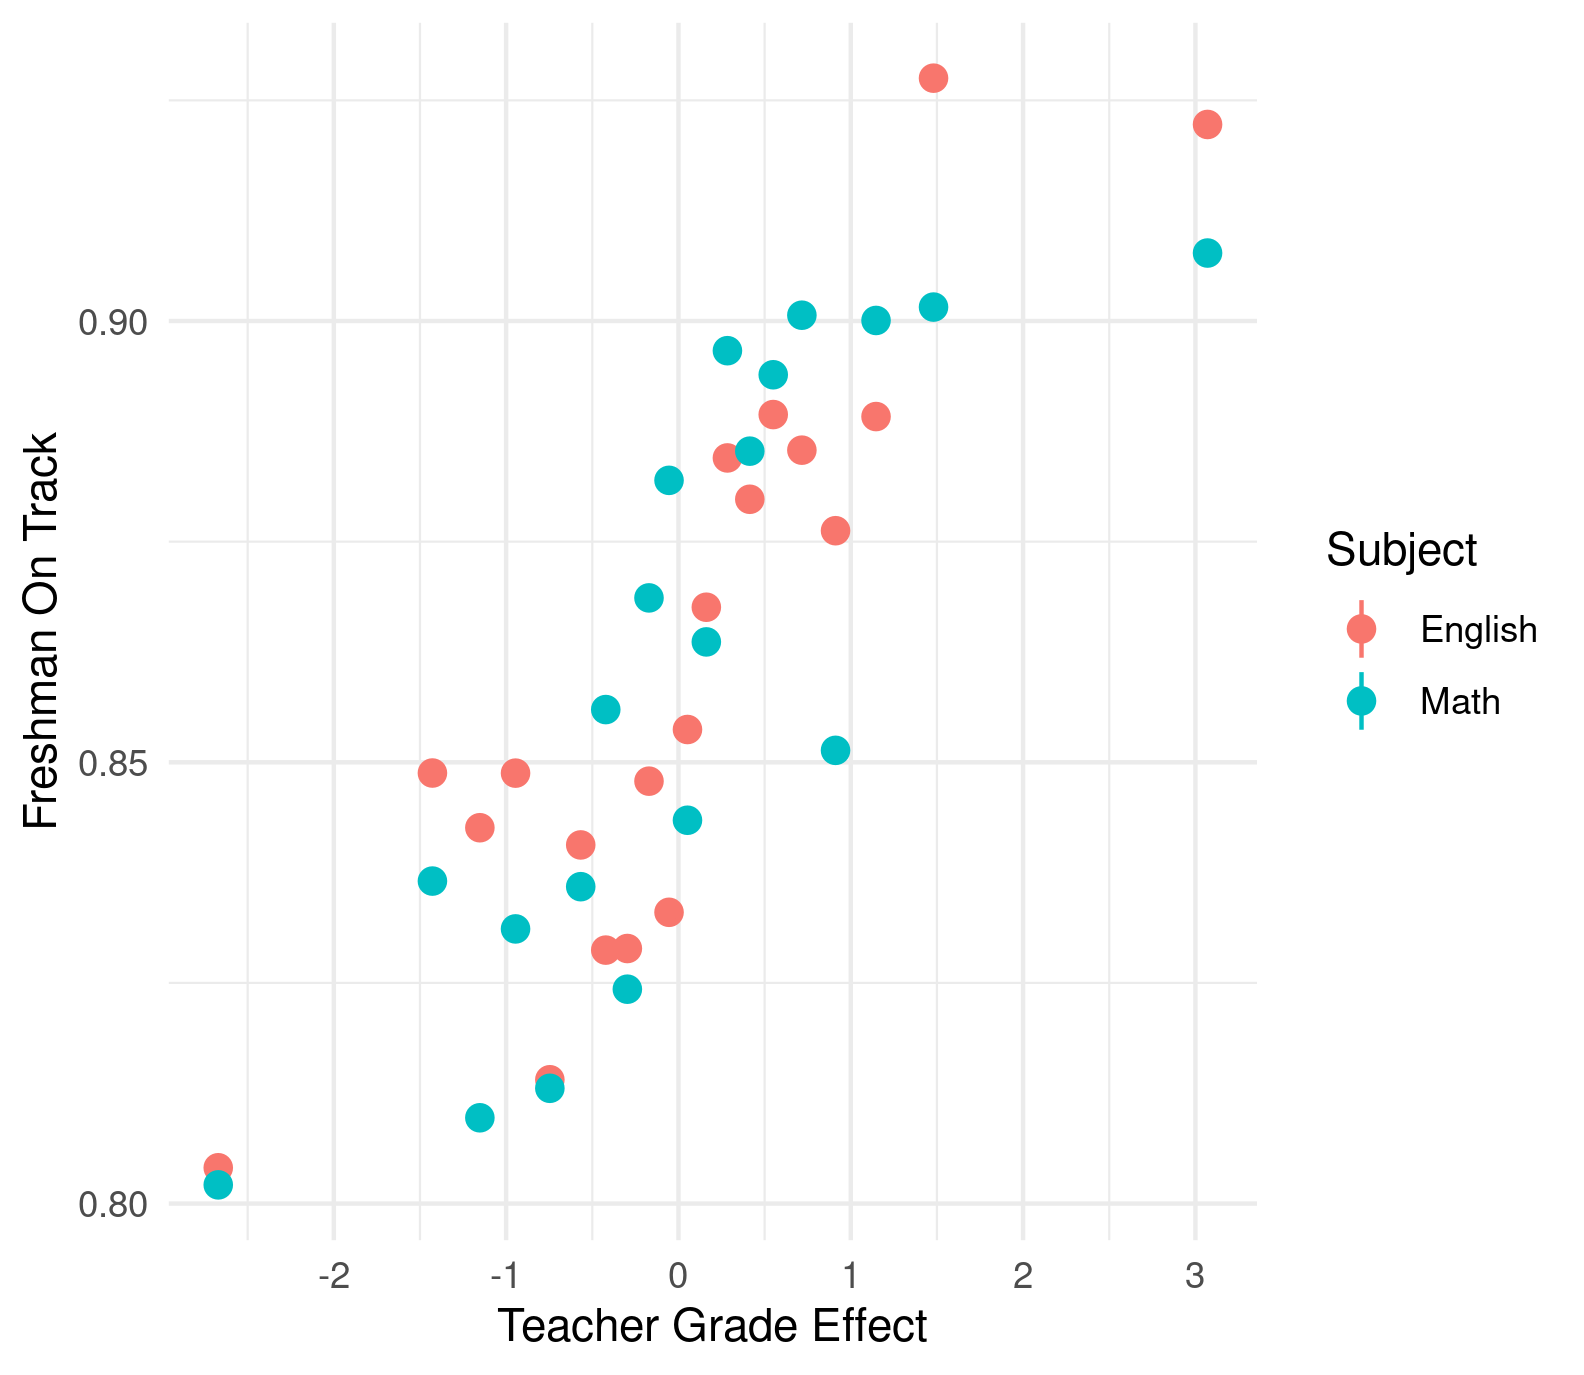
\includegraphics[width=\textwidth]{/Users/roymckenzie/Dropbox/Thesis/ECON/Output/dFreshOnTrack_scatter.png}
         \caption{Freshman on Track}
         \label{fig:dFreshOnTrack}
     \end{subfigure}
     \hfill
     \begin{subfigure}[b]{0.3\textwidth}
         \centering
         \includegraphics[width=\textwidth]{/Users/roymckenzie/Dropbox/Thesis/ECON/Output/freshCoreGpa_scatter.png}
         \caption{Freshman Core GPA}
         \label{fig:freshCoreGpa}
     \end{subfigure}
     \hfill
     \begin{subfigure}[b]{0.3\textwidth}
         \centering
         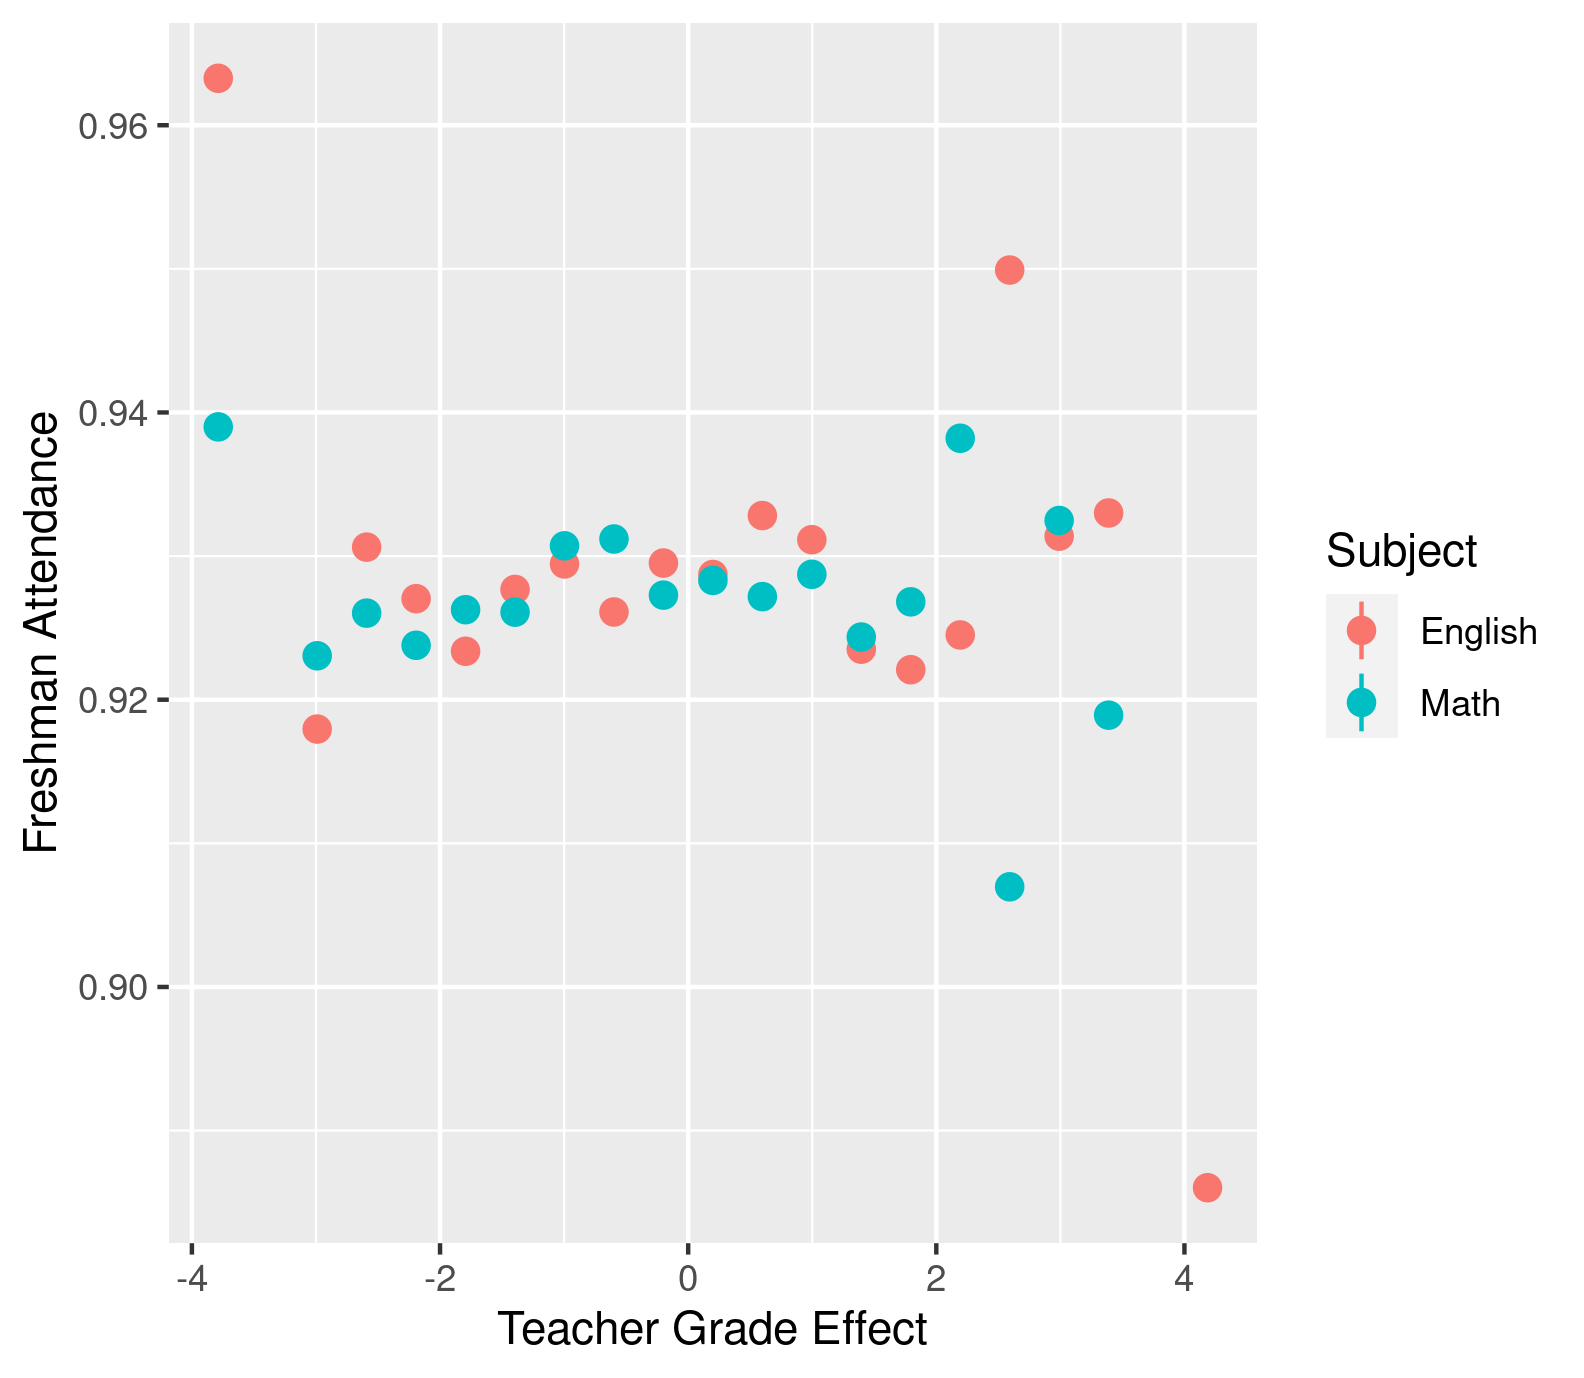
\includegraphics[width=\textwidth]{/Users/roymckenzie/Dropbox/Thesis/ECON/Output/pFreshAttendance_scatter.png}
         \caption{Freshman Attendance}
         \label{fig:pFreshAttendance}
     \end{subfigure}
        \caption{Freshman Year Outcomes}
        \label{fig:fresh}
\end{figure}


\end{frame}


\begin{frame}
\frametitle{Links to Freshman Outcomes}

\begin{figure}
     \centering
     \begin{subfigure}[b]{0.3\textwidth}
         \centering
         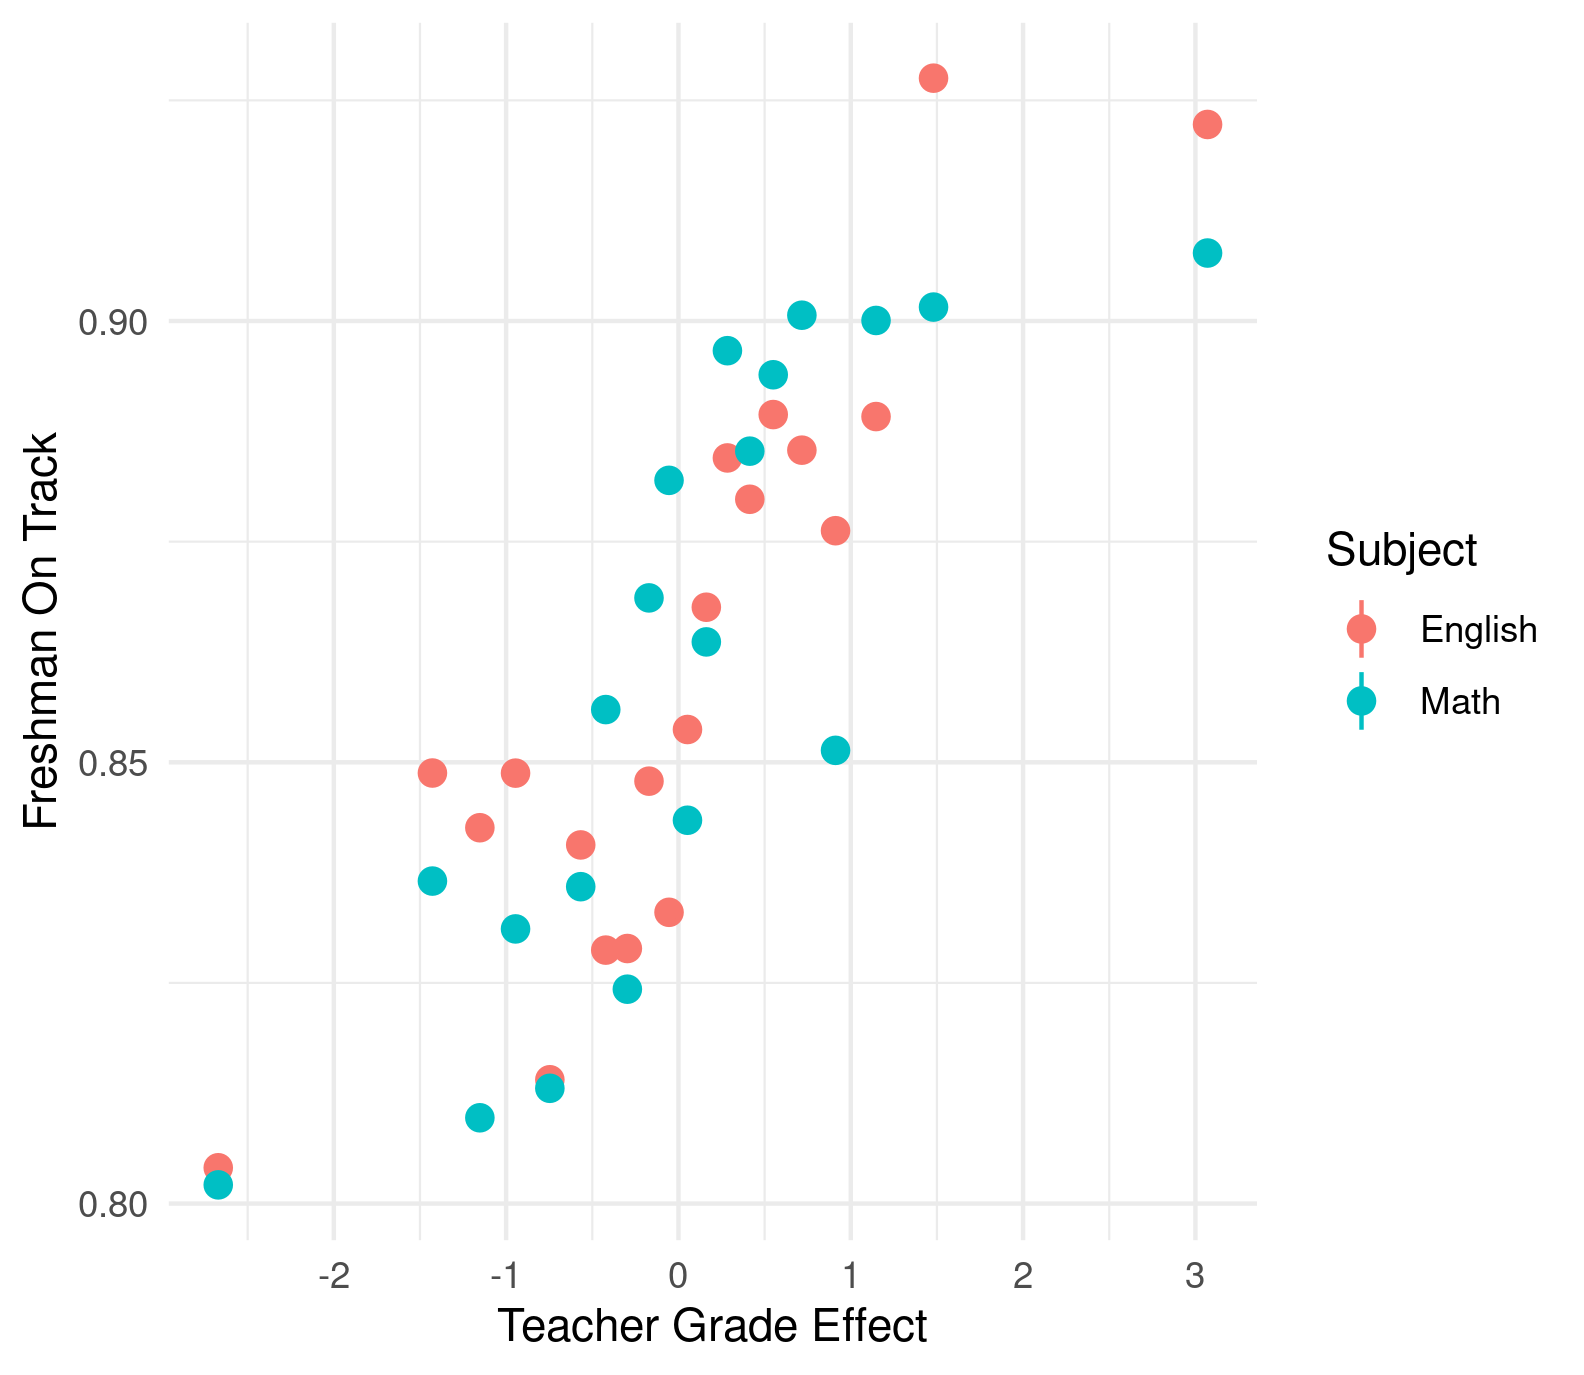
\includegraphics[width=\textwidth]{/Users/roymckenzie/Dropbox/Thesis/ECON/Output/dFreshOnTrack_scatter.png}
         \caption{Freshman on Track}
         \label{fig:dFreshOnTrack}
     \end{subfigure}
     \hfill
     \begin{subfigure}[b]{0.3\textwidth}
         \centering
         \includegraphics[width=\textwidth]{/Users/roymckenzie/Dropbox/Thesis/ECON/Output/freshCoreGpa_scatter.png}
         \caption{Freshman Core GPA}
         \label{fig:freshCoreGpa}
     \end{subfigure}
     \hfill
     \begin{subfigure}[b]{0.3\textwidth}
         \centering
         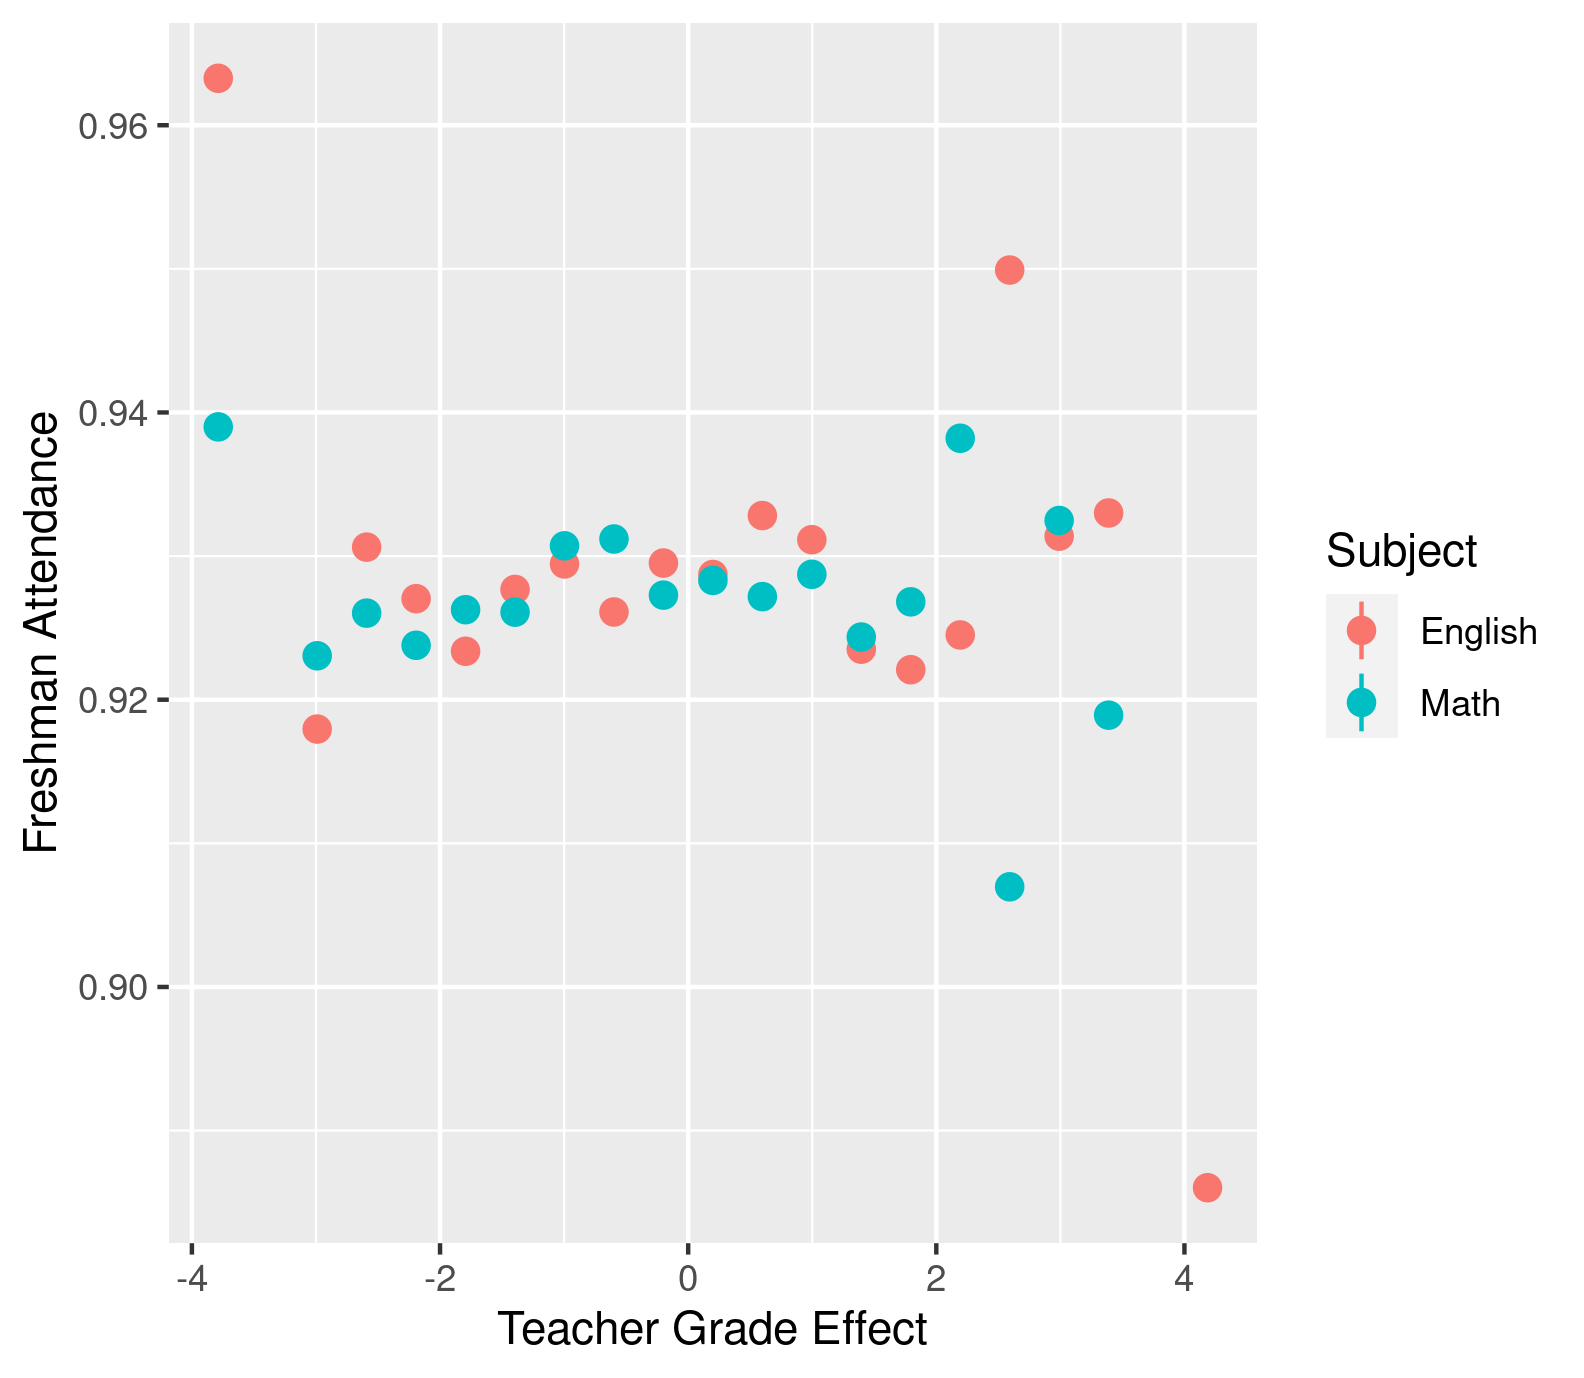
\includegraphics[width=\textwidth]{/Users/roymckenzie/Dropbox/Thesis/ECON/Output/pFreshAttendance_scatter.png}
         \caption{Freshman Attendance}
         \label{fig:pFreshAttendance}
     \end{subfigure}
        \caption{Freshman Year Outcomes}
        \label{fig:fresh}
\end{figure}


\end{frame}


\begin{frame}
\frametitle{Links to Course Taking Outcomes (After Freshman Year)}

\begin{figure}
     \centering
     \begin{subfigure}[b]{0.48\textwidth}
         \centering
         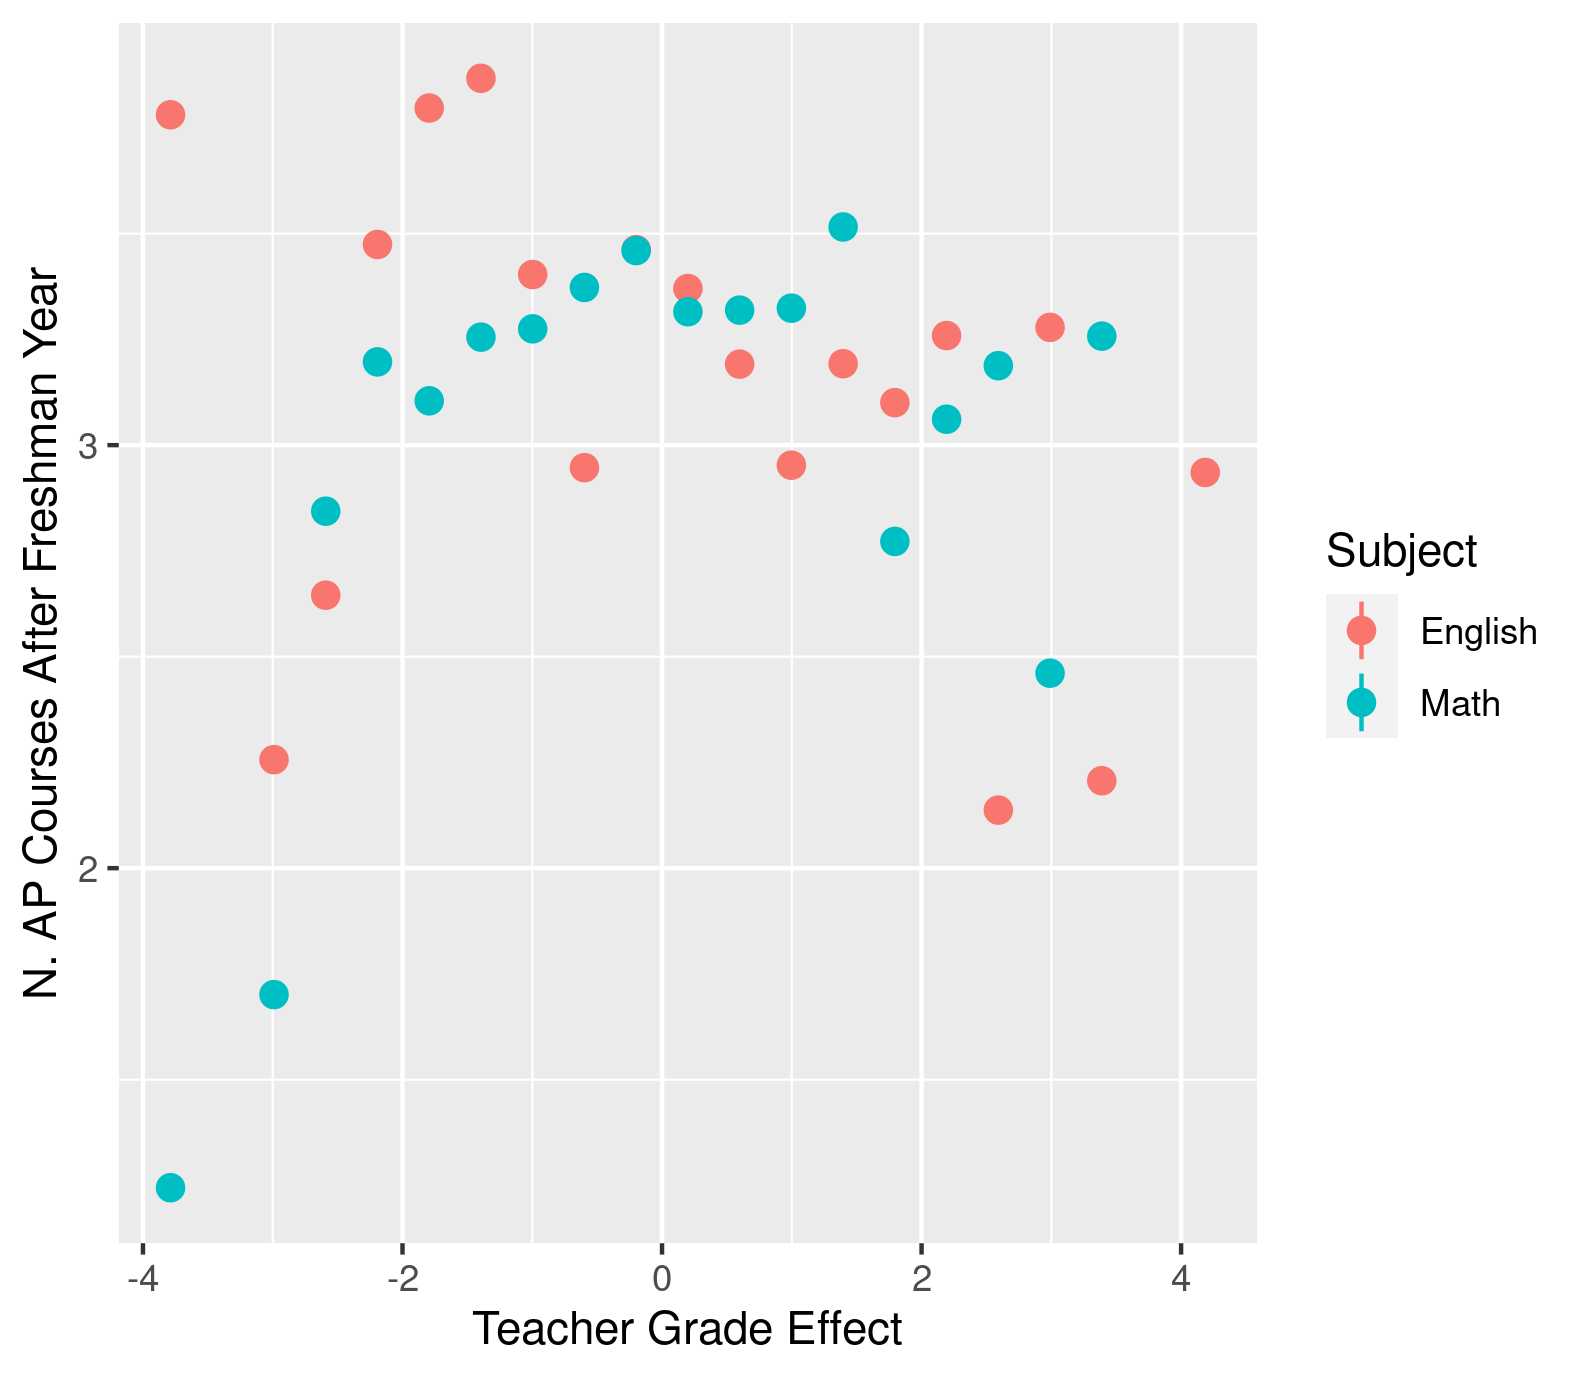
\includegraphics[width=\textwidth]{/Users/roymckenzie/Dropbox/Thesis/ECON/Output/nAPCourses4yr_scatter.png}
         \caption{N. AP Courses}
         \label{fig:nAPCourses4yr}
     \end{subfigure}
     \begin{subfigure}[b]{0.48\textwidth}
         \centering
         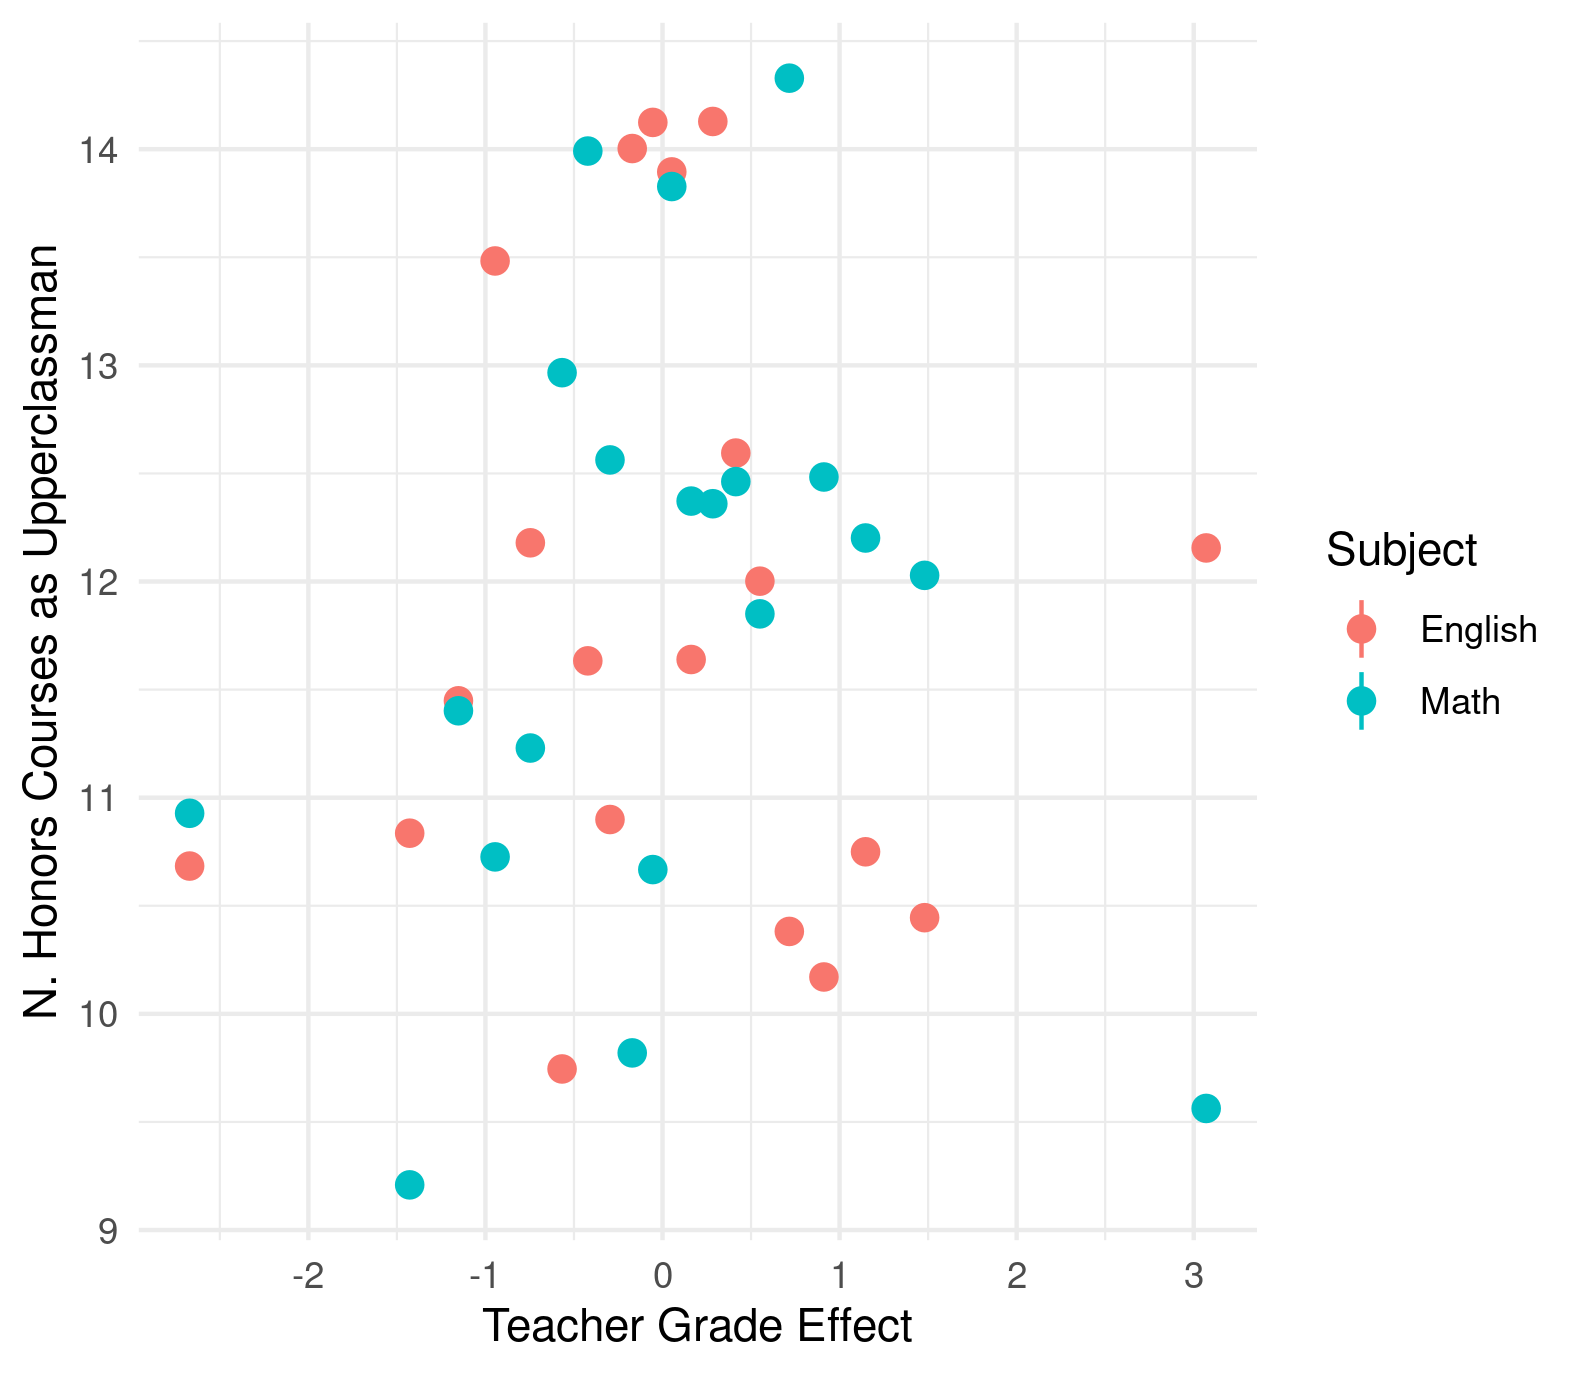
\includegraphics[width=\textwidth]{/Users/roymckenzie/Dropbox/Thesis/ECON/Output/n_honors_after_fresh_scatter.png}
         \caption{N. Honors Courses}
         \label{fig:freshCoreGpa}
     \end{subfigure}
      \caption{Course Taking Outcomes}
      \label{fig:course}
\end{figure}
\end{frame}





\end{document}